\documentclass{report}

\input{~/dev/latex/template/preamble.tex}
\input{~/dev/latex/template/macros.tex}

\title{\Huge{}}
\author{\huge{Nathan Warner}}
\date{\huge{}}
\pagestyle{fancy}
\fancyhf{}
\lhead{Warner \thepage}
\rhead{}
% \lhead{\leftmark}
\cfoot{\thepage}
%\setborder
% \usepackage[default]{sourcecodepro}
% \usepackage[T1]{fontenc}
\usetikzlibrary{graphs,graphs.standard}


\begin{document}
    % \maketitle
        \begin{titlepage}
       \begin{center}
           \vspace*{1cm}
    
           \textbf{Discrete Structures} \\ 
           Graph Theory
    
           \vspace{0.5cm}
            
                
           \vspace{1.5cm}
    
           \textbf{Nathan Warner}
    
           \vfill
                
                
           \vspace{0.8cm}
         
           
\includegraphics[width=0.4\textwidth]{~/niu/seal.png}
                
           Computer Science \\
           Northern Illinois University\\
           August 31, 2023 \\
           United States\\
           
                
       \end{center}
    \end{titlepage}
    \tableofcontents
    \pagebreak \bigbreak \noindent
    \section{\LARGE Graphs}
    \smallbreak \noindent
    \begin{definition}
    \textbf{ A \textbf{graph} $G$ consists of two finite sets: a nonempty set $V(G)$ of vertices and a set $E(G)$ of edges, where each edge is associated with a set consisting of either one or two vertices called its endpoints. Formally, a \textbf{graph} is defined as an ordered pair $G = (V,E)$, where $V$ is the set of vertices and $E$ is the set of edges
        \begin{align*}
            G = (V,E) \\
            V = \{v_{1},v_{2},v_{3},...,v_{n}\} \\
            E = \{e_{1}, e_{2}, e_{3}, ..., e_{m}\}
        .\end{align*}
} 
    \end{definition}
    \bigbreak \noindent 
    \begin{minipage}{0.47\textwidth}
        \incfig{graph1}
    \end{minipage}
    \begin{minipage}{0.47\textwidth}
    \begin{align*}
        V = \{v_{1},v_{2}, v_{3}, v_{4}\} \\
        E = \{e_{1}, e_{2},e_{3},e_{4},e_{5}\}
    .\end{align*}
    We can also represent the edges by only stating the vertices which connect the edges
        \begin{center}
        \begin{tabular}{|l|c|}
        \hline
        Edges & Endpoints \\
        	\hline
        $e_{1}$& $\{v_{1},v_{2}\} $   \\
        	\hline
        $e_{2}$ & $\{v_{1}, v_{3}\} $ \\
        \hline
        $e_{3}$ & $\{v_{2}, v_{3}\} $ \\
        \hline 
        $e_{4}$ & $\{v_{3}, v_{4}\} $ \\
        \hline
        $e_{5}$ & $\{v_{4}\} $ \\
        \hline
        \end{tabular}
    \end{center}
    \end{minipage}

    \pagebreak \bigbreak \noindent 
    \section{\LARGE Subgraphs}
    \smallbreak \noindent
    \begin{definition}
    \textbf{ Graph $H$ is said to be a \textbf{subgraph} of a graph $H$ iff every vertex in $H$ is also a vertex in $G$, every edge in $H$ is also an edge in $G$, and every edge in $H$ has the same endpoints as it has in $G$.} 
    \bigbreak \noindent 
    \end{definition}
    \bigbreak \noindent 
    Consider the graph:
    \bigbreak \noindent 
    \begin{figure}[ht]
        \centering
        \incfig{take45}
        \label{fig:take45}
    \end{figure}
    \bigbreak \noindent 
    Then the possible \textbf{sub graphs} could be:
    \bigbreak \noindent 
    \begin{figure}[ht]
        \centering
        \incfig{tryagain3}
        \label{fig:tryagain3}
    \end{figure}
    \bigbreak \noindent 
    \nt{These graphs are not \textbf{all} the possibilites, just a few.}

    \pagebreak \bigbreak \noindent 
    \section{\LARGE Degree}
    \bigbreak \noindent 
    \smallbreak \noindent
    \begin{definition}
    In graph theory, the \textbf{degree} of a vertex refers to the number of edges that are connected to that vertex. 
    \end{definition}
    \smallbreak \noindent
    \begin{definition}
        \textbf{Parallel edges} are two or more edges that have the same pair of end vertices. 
    \end{definition}
    \smallbreak \noindent
    \begin{definition}
         \textbf{Multiple Edges} is a term used interchangeably with parallel edges. 
    \end{definition}
    \smallbreak \noindent
    \begin{definition}
         An \textbf{isolated vertex} is a vertex that has a degree of zero
    \end{definition}
    \smallbreak \noindent
    \begin{definition}
         A \textbf{loop} is an edge that connects a vertex to itself. 
    \end{definition}
    \smallbreak \noindent
    \begin{definition}
         A \textbf{Degree Sequence} is an \textbf{n-tuple} of the degrees on vertices, in increasing order and with repetition. 
    \end{definition}
    \smallbreak \noindent
    \begin{definition}
         The \textbf{overall degree} is the sum of all the degrees.
    \end{definition}




    \bigbreak \noindent 
    \begin{center}
        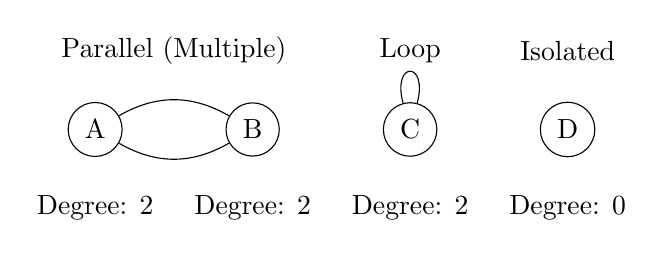
\begin{tikzpicture}
    % Nodes
    \node[draw, circle] (A) at (0,0) {A};
    \node[draw, circle] (B) at (2,0) {B};
    \node[draw, circle] (C) at (4,0) {C};
    \node[draw, circle] (D) at (6,0) {D};
    
    % Edges and Loop
    \draw (A) to[bend left] (B);
    \draw (B) to[bend left] (A);
    \draw (C) to[loop above] (C);
    
    % Labels
    \node at (1,1) {Parallel (Multiple)};
    \node at (4,1) {Loop};
    \node at (6,1) {Isolated};
    
    % Degrees
    \node at (0,-1) {Degree: 2};
    \node at (2,-1) {Degree: 2};
    \node at (4,-1) {Degree: 2};
    \node at (6,-1) {Degree: 0};
\end{tikzpicture}
    \end{center}

    \pagebreak \bigbreak \noindent 
    \section{\LARGE Sum of Degrees and Vertices Theorem}
    \smallbreak \noindent
    \begin{definition}
    \textbf{To denote the number of vertices in a graph, we say $||V||$, or just $|v|$}. To denote the number of edges in a graph, we say $||E||$, or just $|E|$ 
    \end{definition}
    \smallbreak \noindent
    \begin{definition}
    The number of vertices in a graph is called the \textbf{order} of the graph
    \end{definition}
    \smallbreak \noindent
    \begin{definition}
     The number of edges in a graph is called the \textbf{size} of the graph.
    \end{definition}
    \bigbreak \noindent 
    Consider the graphs:
    \bigbreak \noindent 

    \begin{minipage}{0.47\textwidth}
        \incfig{graphe}
    \end{minipage}
    \begin{minipage}{0.47\textwidth}
    Then we have:
    \begin{align*}
        ||V|| = 4 \\
        ||E|| = 5 \\
        \sum\ deg = 10
    .\end{align*}
    %\caption{}
    %\label{fig:}
    \end{minipage}
    \bigbreak \noindent 
    \begin{minipage}{0.47\textwidth}
        \incfig{graphee}
    %\caption{}
    %\label{fig:}
    \end{minipage}
    \begin{minipage}{0.47\textwidth}
        \begin{align*}
            ||V|| = 3 \\
            ||E|| = 6\\
            \sum\ deg = 12
        .\end{align*}
    %\caption{}
    %\label{fig:}
    \end{minipage}
    \bigbreak \noindent 
    So you might notice from these two examples that the total degree of the graph ($\sum\ deg$) is exactly \textbf{twice} the number of edges. Thus, we can conclude:
    \bigbreak \noindent 
    \pagebreak \bigbreak \noindent  
    \begin{thrm}
       \begin{align*}
           \sum\ deg = 2||E||
       .\end{align*} 
    \end{thrm}
    \bigbreak \noindent 
    \begin{proof}
       Let $G$ be a graph, that has $n$ vertices $v_{1},v_{2},v_{3},v_{4},...,v_{n}$ and $m$ edges, where $n$ is a positive integer and $m$ is a nonnegative integer.
       \bigbreak \noindent 

       If $e_{1}$ is an edge, then 
          \begin{equation}
           v_{i},v_{j}=
               \begin{cases}
                     1\ edge,\ 1V & \rightarrow degree = 2  \\
                    1\ edge,\ 2V & \rightarrow degree =  2  
               \end{cases}
           \end{equation}
           \bigbreak \noindent 

        Thus, no matter the case, the edge always contributes 2 to the total degree.
    \end{proof}
    \bigbreak \noindent 
    \begin{corr}
      The total degree of a graph is even. 
    \end{corr}
    \smallbreak \noindent
    \begin{corr}
       In any graph, there are an even number of vertices of odd degree.
    \end{corr}

    \pagebreak \bigbreak \noindent 
    \section{\LARGE Adjacency and Incidence}
    \smallbreak \noindent
    \begin{definition}
        \textbf{vertices that are connected by an edge are  \textbf{adjacent}} 
    \end{definition}
    \smallbreak \noindent
    \begin{definition}
        \textbf{A vertex with a loop is \textbf{adjacent to itself}} 
    \end{definition}
    \smallbreak \noindent
    \begin{definition}
        \textbf{Two edges that share a vertex are \textbf{adjacent}} 
    \end{definition}
    \smallbreak \noindent
    \begin{definition}
        \textbf{An edge is \textbf{incident} on its endpoints} 
    \end{definition}
    \smallbreak \noindent
    \begin{definition}
    \textbf{A vertex on which no edges are incident is an \textbf{isolated vertex.}} 
    \end{definition}

    \pagebreak \bigbreak \noindent 
    \section{\LARGE Adjacency Matrix}
    \bigbreak \noindent 
    \smallbreak \noindent
    \begin{definition}
        Let $G $ be a graph with vertices labeled $\{1,2,3,...,n\} $. Then the \textbf{Adjacency Matrix} of $G$ is the $n \times n$ matrix whose $ij^{th}$ term is the number of the edges joining vertex $i $ and vertex $j $
    \end{definition}
    \bigbreak \noindent 
    Consider the graph:
    \bigbreak \noindent 
    \begin{minipage}{0.47\textwidth}
        \incfig{grapher1}
    \end{minipage}
    \begin{minipage}{0.47\textwidth}
    Since we have 5 vertices, then we will have a $5 \times 5$ matrix. Thus, our matrix for this graph will be:

    \begin{align*}
        A = \begin{bmatrix}
            0 & 1 & 0 & 0 & 0 \\
            1 & 0  & 2 & 0 & 1 \\
            0 & 2 & 0 & 0 & 0  \\
            0 & 0 & 0 & 1 & 1 \\
            0 & 1 & 0& 1 & 0 
        \end{bmatrix}
    .\end{align*}
    To make things clearer, here is how the rows and columns are labeled:
            \[
    \begin{array}{c|ccccc}
     & v_1 & v_2 & v_3 & v_4 & v_5 \\
    \hline
    v_1 & 0 & 1 & 0 & 0 & 0 \\
    v_2 & 1 & 0 & 2 & 0 & 1 \\
    v_3 & 0 & 2 & 0 & 0 & 0 \\
    v_4 & 0 & 0 & 0 & 1 & 1 \\
    v_5 & 0 & 1 & 0 & 1 & 0 \\
    \end{array}
    \]
    \end{minipage}

    \pagebreak \bigbreak \noindent 
    \section{\LARGE Incidence Matrix}
    \smallbreak \noindent
    \begin{definition}
        \item An \textbf{incidence matrix} is a rectangular matrix \( B \) where \( B[i][j] \) represents the relationship between vertex \( i \) and edge \( j \).

    \end{definition}
    \bigbreak \noindent 
    Suppose we have the graph:
    \bigbreak \noindent 
    \begin{minipage}[]{0.47\textwidth}
        \incfig{figher}
    \end{minipage}
    \begin{minipage}[]{0.47\textwidth}
       Then we write the \textbf{incidence matrix} as follows:
       \begin{align*}
          M = \begin{bmatrix}
               1 & 1 & 0 & 0 & 2 \\
               0 & 1 & 0 & 1 & 0 \\
               0 & 0 & 1 & 0 & 0  \\
               1 & 0 & 1 & 1 & 0 
           \end{bmatrix}
       .\end{align*}
       Where the vertices as labeled vertically, and the edges are labeled horizontally, as such:
       \bigbreak \noindent 
        \[
        \begin{array}{c|ccccc}
            & e_{1} & e_{2} & e_{3} & e_{4} & e_{5} \\
        \hline
            v_{1} & 1 & 1 & 0 & 0 & 2 \\
            v_{2} & 0 & 1 & 0 & 1 & 0 \\
            v_{3} & 0 & 0 & 1 & 0 & 0  \\
            v_{4} & 1 & 0 & 1 & 1 & 0 
        \end{array}
        \]
    \end{minipage}

    \pagebreak \bigbreak \noindent 
    \section{\LARGE Isomorphism}
    \smallbreak \noindent
    \begin{definition}
        Two graphs G1 and G2 are isomorphic if they have the same number of vertices, edges, and there exists a matching between their vertices so that two vertices are connected by an edge in G1 if and only if corresponding vertices are connected by an edge in G2.
    \end{definition}
    \bigbreak \noindent 
    Consider the graphs:
    \bigbreak \noindent 
    \begin{minipage}[]{0.47\textwidth}
        \incfig{iso}
    \end{minipage}
    \begin{minipage}[]{0.47\textwidth}
       \incfig{iso2}
    \end{minipage}
    \bigbreak \noindent 
    We can then see that these two graphs are \textbf{isomorphic}
    \bigbreak \noindent 

    \pagebreak \bigbreak \noindent 
    \section{\LARGE Walks, Trails, Paths, and Circuits}
    \bigbreak \noindent 
    \begin{definition}
    For the graph $G$, and vertices $V$ and $W$, a \textbf{walk} from $V$ to $W$ is a finite alternating sequence of adjacent vertices and edges of $G$ \\
    The \textbf{length} of a walk is the number of edges in the walk. \\
    A \textbf{trivial walk} is a walk with length zero. \\
    A \textbf{closed walk} is a walk that starts and ends at the same vertex \\
    An \textbf{open walk} is a walk that starts and ends at different vertices 
    \end{definition}
    \bigbreak \noindent 
    Suppose we have the graph:
    \bigbreak \noindent 
    \begin{minipage}[]{0.47\textwidth}
        \incfig{walk}
    \end{minipage}
    \begin{minipage}[]{0.47\textwidth}
        Then we can say a possible walk from 1 to 2 could be:
        \begin{align*}
           W = 1\ e\ 5\ h\ 4\ g\ 2 
        .\end{align*}
    \end{minipage}
    \bigbreak \noindent 
    \begin{definition}
        A \textbf{Trail} from $v$ to $w$ is a walk from $v$ to $w$ that does not contain a repeated edge.
    \end{definition}
    \bigbreak \noindent 
    \smallbreak \noindent
    \begin{definition}
        A \textbf{Path}  from $v$ to $w$ is a trail that does not contain a repeated vertex. So, by inheritance, a path can also have \textbf{no} repeated edges. \\
       The \textbf{distance} between two vertices is the length of the shortest path between those two vertices
       \begin{align*}
           d(v_{1},v_{2})
       .\end{align*}
    \end{definition}
    \bigbreak \noindent 
    \begin{definition}
        A \textbf{Circuit}  is a trail that contains at least one edge and starts and ends at the same vertex
    \end{definition}

    \pagebreak \bigbreak \noindent 
    \section{\LARGE Eccentricity, Diameter, and Radius}
    \bigbreak \noindent 
    \smallbreak \noindent
    \begin{definition}
          \item The \textbf{Eccentricity} of a vertex is the distance from $v$ to a vertex farthest from $v$
      \begin{align*}
          ecc(v) \\ 
          or:\ e(v)
        .\end{align*}
    \end{definition}
    \bigbreak \noindent 
    Consider the graph:
    \bigbreak \noindent 
    \begin{minipage}{0.47\textwidth}
        \incfig{eccen}
    \end{minipage}
    \begin{minipage}{0.47\textwidth}
        Thus we have:
        \begin{align*}
            d(1,2) = 1 \\
            d(1,3) = 1 \\
            d(1,4) = 2\\ 
            d(1,5) =  3
        .\end{align*}
        From these observations, we can deduce:
        \begin{align*}
            ecc(1) = 3 \\
            ecc(2) = 2 \\
            ecc(3) = 3 \\
            ecc(4) = 2 \\
            ecc(5) = 3
        .\end{align*}
    \end{minipage}
    \bigbreak \noindent 
    \smallbreak \noindent
    \begin{definition}
       The \textbf{diameter} of a graph $G$ is the maximum vertex eccentricity. \\
       The \textbf{radius} of a graph $G$ is the minimum vertex eccentricity. \\
         If $ecc(v)  = diam(G)$, then $v$ is a \textbf{peripheral vertex} \\
       If $ecc(v) = rad(G)$, then $v$ is a \textbf{central vertex}
    \end{definition}

    \pagebreak \bigbreak \noindent 
    \section{\LARGE Connectedness}
    \bigbreak \noindent 
    \smallbreak \noindent
    \begin{definition}
        \begin{itemize}
            \item A \textbf{graph is connected} iff there is a walk between each pair of vertices
            \item A \textbf{disconnecting set} for a graph $G$ is a set of edges whose removal disconnects $G$  
            \item A \textbf{cut set} is a disconnecting set such that no proper subset of the disconnecting set is disconnecting 
            \item A \textbf{bridge} is a disconnecting set that has a cardinality of 1 
            \item \textbf{Edge connectivity} represents  the minimum number of edges that you have to remove such that you get the graph to be disconnected
            \begin{align*}
                \text{Edge connectivity: } \lambda(G)
            .\end{align*}
        \item A \textbf{separating set} is a set of vertices whos removal will cause a disconnection in the graph. 

            \textbf{Note:} Deletion of a vertex in a graph will also remove any edges that are connected to that vertex. 
        \item A \textbf{cut-vertex} is a vertex whose removal causes the graph to be disconnected and split into components 
        \item \textbf{Vertex connectivity} is the minimum number of vertices that must be removed to cause a disconnection.
            \begin{align*}
                \text{Vertex connectivity: } \kappa(G)
            .\end{align*}
        \end{itemize}
    \end{definition}

    \pagebreak \bigbreak \noindent 
    \section{\LARGE Euler Trails and Circuits}
    \bigbreak \noindent 
    \smallbreak \noindent
    \begin{definition}
        \begin{itemize}
            \item  An \textbf{Euler trail} is a trail that visits every edge exactly once.
            \item \textbf{If all vertices have even degrees except two, we can declare that the graph has a Euler trail}
            \item An \textbf{Euler circut} is an Euler trail that visits every edge exactly once and starts and ends at the same vertex.
            \item \textbf{If all vertices have even degrees then we have an Euler circuit}
            \item A connected graph $G$ is \textbf{Eulerian} iff the degree of each vertex is even
        \end{itemize}
    \end{definition}

    \pagebreak \bigbreak \noindent 
    \section{\LARGE Fleury's Algorithm}
    \bigbreak \noindent 
    \smallbreak \noindent
    \begin{definition}
        \textbf{Fleury's algorithm} is an algorithm that is used to find Euler trails and circuits 
    \end{definition}
    \bigbreak \noindent 
    \textbf{Steps (Euler Trail):}
    \begin{enumerate}
        \item Start at odd vertex
        \item Verify that the requirements for an euler trail or circuit are satisfied
        \item Make a replica of the graph
        \item Pick an edge, then delete it from the replica, if the deletion of the edge causes would cause the graph to become disconnected, do not remove the edge.
    \end{enumerate}
    \bigbreak \noindent 
    \textbf{Steps (Euler Circuit):}
    \begin{enumerate}
        \item Start at any vertex
        \item Verify that the requirements for an euler trail or circuit are satisfied
        \item Make a replica of the graph
        \item Pick an edge, then delete it from the replica, if the deletion of the edge causes would cause the graph to become disconnected, do not remove the edge.
    \end{enumerate}

    \pagebreak \bigbreak \noindent 
    \section{\LARGE Hamiltonian paths and circuits}
    \bigbreak \noindent 
    \smallbreak \noindent
    \begin{definition}
        \begin{itemize}
            \item A \textbf{Hamiltonian path} is a path that visits every vertex exactly once  
            \item A \textbf{Hamiltonian circuit} is a circuit that contains each vertex in $G$ exactly once, except for the starting and ending vertex that appears twice.
            \item A \textbf{Hamiltonian graph} is a graph that has a Hamiltonian circuit
        \end{itemize}

    \end{definition}

    \pagebreak \bigbreak \noindent 
    \section{\LARGE Ore's Theorem}
    \bigbreak \noindent 
    \begin{thrm}
       If a simple graph with $n \geq 3$ vertices, and if deg(v) + deg(w) $ \geq n$ for each pair of non-adjacent vertices $v$ and $w$, then $G$ is Hamiltonian 
    \end{thrm}

    \pagebreak \bigbreak \noindent 
    \section{\LARGE The shortest path problem}
    \bigbreak \noindent 
    \smallbreak \noindent
    \begin{definition}
        A \textbf{weighted graph} is a graph whose edges have some weight (value) 
    \end{definition}
    \bigbreak \noindent 
    \subsection{Dijkstran's algorithm}
    \bigbreak \noindent 
    \begin{enumerate}
        \item Pick starting and ending vertices
        \item Give a value of zero to your starting vertex, and give the other vertices a value of infinity
        \item Pick a vertex to travel to from your starting point
        \item Add the weight of the edge to the vertex
        \item If the value is less than the vertex you are traveling to, update it.
        \item Once you travel to all possible vertices that are connected to your starting vertex, you are done with that vertex
        \item Repeat with other vertices 
    \end{enumerate}
    








        





    
    
    
    
    
    

     




\end{document}
